\documentclass[a4paper, 10pt]{article}
\usepackage[cm]{fullpage}
\usepackage{graphicx}
\begin{document}

\title{Software Engineering (Practice) Coursework 3 \\ \textit{busyroute} \\ Product Management, Feedback and Evaluation}
\author{Group 2 (Thomas Burnell, Andrei Cioara, Jeremy Kong, Andrea Michi, Alice Sibold)}
\maketitle

\section{Background}
%TODO Tom, if you want to change this, go ahead.
Individuals often face the problem of having to develop an itinerary for efficiently completing various tasks, many of which can only be done at certain locations. For example, they may have to withdraw cash and meet a friend for coffee during their (short) lunch break. Such an itinerary may be easily planned by one who knows the exact locations he needs to visit, the order in which he should visit them, and their distances from each other / his current position, however triviality vanishes when any of these are unknown. Our project aims to provide a user with a system, named \textit{busyroute}, that can determine a suitable route to complete all of his tasks. This differs from existing routing products in that \textit{busyroute} is intended to be able to cope with planning routes incorporating multiple destinations in an arbitrary order, as well as situations where the exact locations or even types of locations may not necessarily be well-defined. In motivation, consider a user who wants to post a letter and fetch a coffee. Our application could suggest visiting a postbox the user is unaware of in a street closely neighbouring a nearby Starbucks store, rather than venturing to the Post Office he is familiar with, situated farther away.

\section{Stakeholders / Users}
\subsection{Identifying our Stakeholders}
Our product aims to serve the needs of busy people -- people who need to complete a series of tasks in an efficient manner. These tasks include a wide variety of fairly common actions, such as posting a letter or getting a coffee, that people from all walks of life are likely to need or want at some point. Furthermore, we have found that it is fairly common for people to need to complete multiple tasks under time constraints; thus, the potential user base for our application is large and fairly diverse.\\\\
The idea for this product was mooted by our Project Supervisor (PS) Professor Sophia Drossoupoulou; she wanted to find efficient ways of running her errands, whether personal or professional, and fitting them into her busy life as a working professional (in this specific case, an academic). We meet with our PS at least once a week, which allows us to frequently discuss our work as well as the direction of our project with her.\\\\
A second group of users would be students; this may prove advantageous as we have ready access to ourselves as well as to other students in the Department of Computing, and we would thus be able to identify this user group's priorities and key requirements more easily.  From our personal experience, the need to run several errands in a limited time (e.g. during lunch breaks) is not uncommon. \\\\
Finally, a third group of users we intend to target are tourists and frequent travellers. The notion of having a limited time is clearly relevant for these users, as they will generally only be in the location they're visiting for a short time and might want to maximise vacation time. Our team members do have several relatives and personal friends who would fall into this category of users; that said, we are being especially careful to not let them know that we're demoing our own product lest this bias their feedback\footnote{\texttt{http://momtestbook.com/}}.
\newpage
\subsection{Gathering Requirements}
In order to determine the PS's requirements as well as those of fellow working professionals, we held initial planning meetings with her to discuss the overall direction of the project and what she would look for in the final product. Minutes were taken during these meetings to ensure that her requests were suitably considered and followed. Initially, our team had difficulty deciding between two interesting routing problems (as discussed in our first report). We contacted the PS and engaged with her in remote discussion over email to help us come to a decision. We also hold weekly meetings with the PS to ensure that new and changing requirements are recognised; using Agile methods and working with an iterative approach helps us remain flexible with regard to potential changes in requirements (which we have experienced over the course of this project). A concern that the PS raised was that our application would need to be convenient to use -- this is especially relevant for busy people who would otherwise not bother with a routing application.  \\\\
Within our team, we also held internal brainstorming sessions at the beginning of the project, during which we tried to identify problems we faced when addressing the errands we had to run. We drew on our personal experience as students with fairly busy schedules. In addition, we also discussed our ideas with several straight-talking friends and coursemates, who were able to provide valuable feedback and ideas for our application. \\\\
%TODO Touristy stuff
We did not \textit{initially} consider tourists to be one of our major user groups; initially, the main user groups we were targeting were busy working professionals and students. However, we found from our personal experiences with travelling on holiday as well as discussions with relatives and personal friends who are frequent travellers that our application could be useful. In particular, as tourists often come from a wider range of backgrounds than working professionals and students (who tend to be relatively comfortable with technology), a common requirement that many of these users expressed was that our system needs to be not just convenient, but also simple to use. \\\\
%TODO I'm not sure if this should be included???
Thus, we identified a set of key requirements for our project, as follows. These requirements are subject to change, however; and we prioritised them according to our customers' preferences as discussed in section 3.1.
\begin{enumerate}
\item Users should be able to specify one or more tasks (from a pre-defined selection) that they need to complete. \\(These tasks may or may not have specific user-defined locations.)
\item Users should be able to enter information about these tasks through a web UI.
\item Users should find the web UI simple and easy to use.
\item Users should be able to have their tasks mapped to locations where they might be completed.
\item Users should be able to indicate a location from which they begin travelling to possible locations.
\item Users should be given an \textit{optimal} or close to optimal route that incorporates locations such that the user can complete all of his or her tasks. 
\item Users should be presented the output of our algorithm through a web UI.
\item Users should have the output visualised graphically; the PS suggested using the Google Maps API for visualisation.
\end{enumerate}
\newpage
\subsection{Value Proposition}
With these requirements in mind, we constructed a Value Proposition Canvas which helped us reflect on how \textit{busyroute} could help satisfy our users' requirements, and better understand how features we developed would be beneficial for our customers\footnote{``Value proposition canvas template." \texttt{http://www.peterjthomson.com/2013/11/value-proposition-canvas}}. This would also be useful in helping us evaluate the success of our product, as elaborated upon in Section 4.
\begin{center}
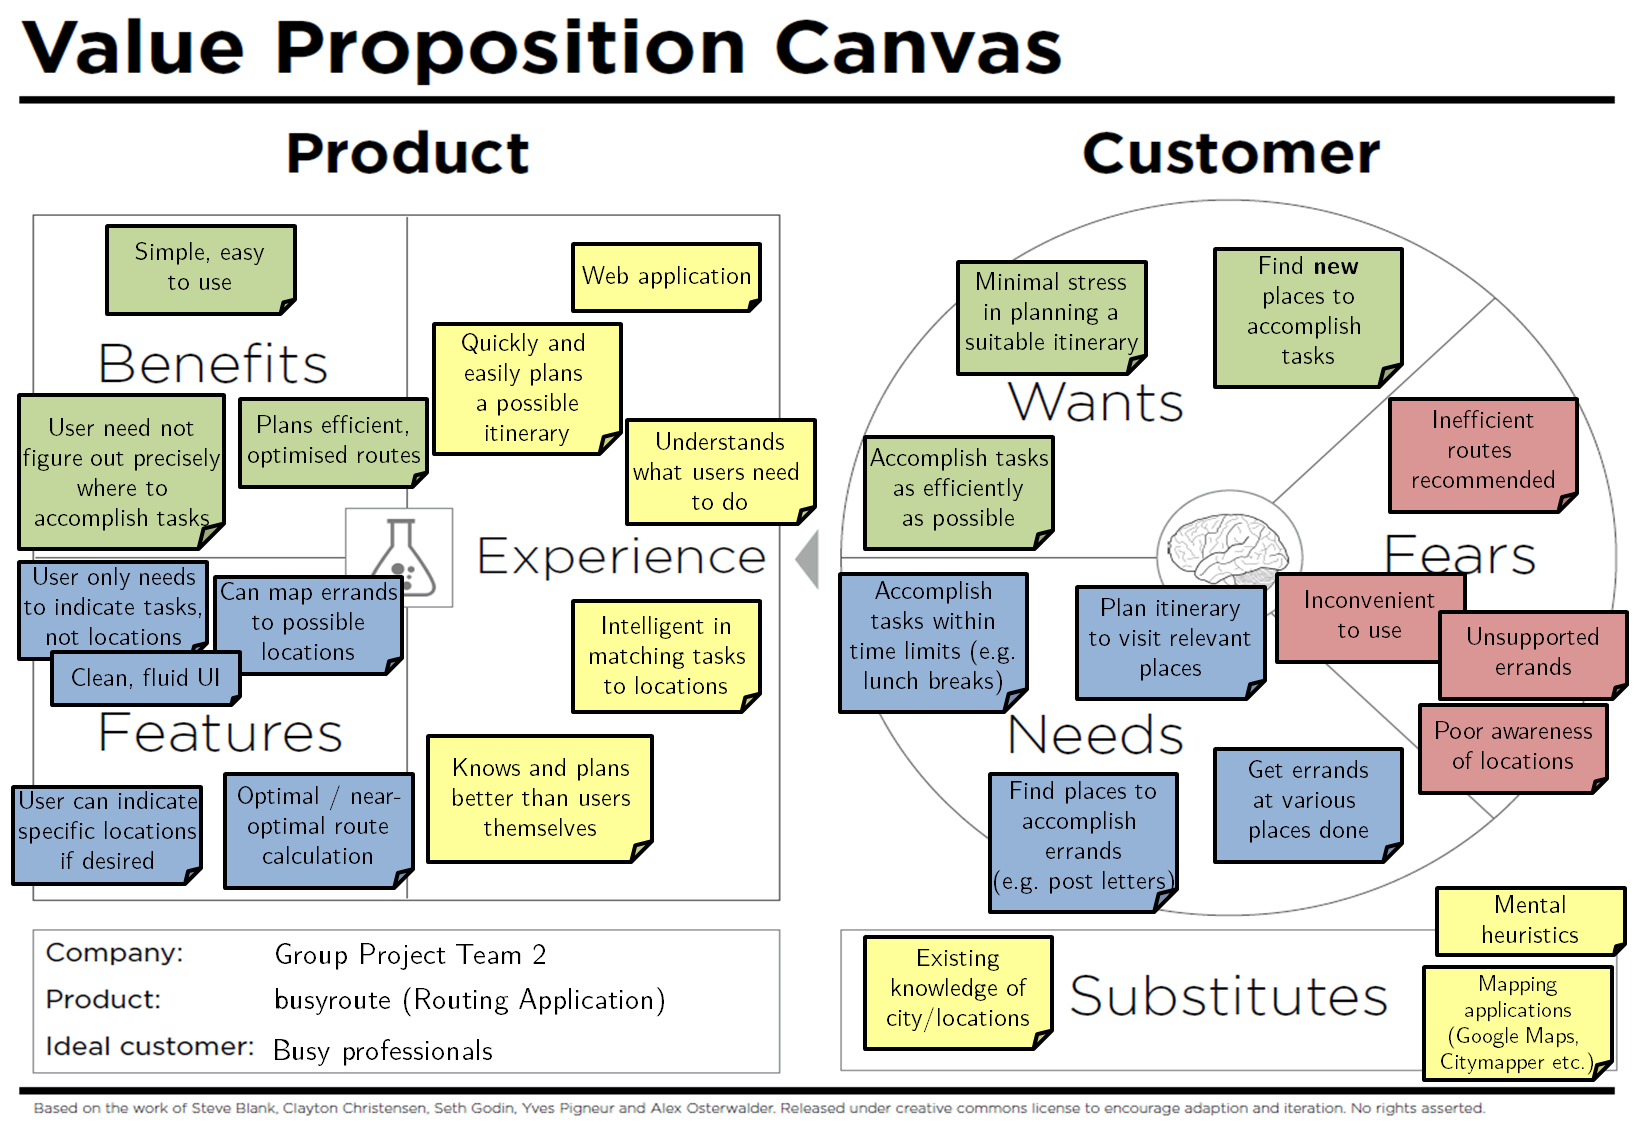
\includegraphics[scale=0.66]{vpc.png} \\
Figure 1. \textit{busyroute} Value Proposition Canvas.
\end{center}

\section{Feedback}
We are building our application in an agile fashion: we work through short, time-boxed iterations, and between each user requirements can be added, modified and re-prioritised. As such, the more feedback we are able to obtain, the more confident we can be in the direction in which we head. Our many aforementioned stakeholders provide us with many sources of such feedback, both in terms of how our product is evolving, as well as how we are working as a team. Throughout this section we will explain how we gather and use both types of feedback.
\subsection{Product Feedback}
\subsubsection{Gathering Feedback}
We hold different types of relationships with our various stakeholders, and so our methods of gathering feedback among them vary. With our PS, we hold weekly Sprint Demo meetings, where we demonstrate the result of our work through the terminating iteration. Here, the PS offers her opinion on what we have done, compares our work to her brief from the previous week's meeting, and outlines the direction in which she would like us to head during the next iteration. \\\\
We wanted a way to be able to demonstrate specific versions of our application to a wider group of critics. Using our development environments to demonstrate this proved to be somewhat difficult, and so we set up multiple so-called demo environments. These are Imperial DoC CloudStack-hosted environments, which specific versions of our application are pushed to. This provides us with a simple way for all team members to access the same specific version(s), without needing to affect his local workspace. Using these environments, we have carried out hallway testing with other students (a key subset of our target user base of “busy people”), as well as cross-validation among team members. We considered the possibility of carrying out A/B testing, using our multiple demo environments. However, since our sample size is likely to be very limited (owing to time, manpower and budget constraints), we determined that it would be difficult to make statistically significant observations, and so didn't carry out this form of testing. \\\\
Following our Sprint Demo each week, we carry out a Sprint Planning meeting, which typically lasts for about 2 hours. Officially, Scrum would require the PS to be present\footnote{\texttt{http://scrummethodology.com/scrum-meetings/}}, however due to their busy schedules they are unable to be. Therefore, we gather as much feedback as possible in the Demo meeting to take through to Planning, and we also email the PS with a detailed report of our Planning meeting outcome, for approval before development begins.\\\\
We wanted to be able to collect comparable feedback from a wide group of users (perhaps beyond those we could reach with hallway testing), in order to identify different and mutual requirements and preferences. Our PS suggested that one way of collecting such feedback would be to design a script which, along with an appropriately configured demo environment, team members could use to individually and remotely gather customer responses. Please refer to Appendix A to see this survey.\\\\
We are unable to have regular meetings with our other stakeholders. To prevent this from being problematic, the PS suggested that we design a prototype in the form of a slide deck, which we could present to various customers. Our prototype is designed to show the entire length of a user story. Please refer to Appendix B to see this prototype.\\\\
Finally, we have a comprehensive test suite, whose run is automated on each build and prior to deployment. The results of this test run provide us with feedback from the system, which helps us to ensure correctness, avoid regressions, and minimise the time and cost of debugging.
\subsubsection{Using Feedback for Improvement}
We don't just gather feedback for feedback's sake, but rather we obsessively use it to improve our product and workflow. Firstly, we use our feedback to prioritise our features. As mentioned in our previous report, we use Trello\footnote{An online project management application, which we use to manage our story board; see \texttt{http://www.trello.com}} for managing the flow of tasks from their origin in the Product Backlog through to being deemed as Done. It is the first of these columns -- the Product Backlog -- which is most directly influenced by our feedback. We keep this column strictly ordered, according to our customers' preferences. Our application is very complex and consists of many layers algorithmically. During an early Demo meeting, our PS voiced preference for us to implement the optimal routing functionality of our application, using a set of given points to visit, before implementing the translation of high-level user errands to places where such errands can be completed. As we generally select the highest priority item(s) from the Product Backlog to work on during an iteration, this helps drive our Sprint plans as well.
\\\\
Our feedback from our customers and PS in particular help us to determine if we are building the right thing. Since our Sprints are just one week long, we are able to demonstrate a stable version of our product weekly, and gather specific and detailed feedback. This frequency helps us to reduce the amount of work potentially wasted, should we have implemented functionality not in line with the PS' expectations or requirements.
\\\\
Finally, we use our feedback to minimise the time and cost of debugging code. Our automated test suites allow us to gather correctness and regression feedback from the system on each build/deploy. This frequent running of our tests results in very small windows during which code can become broken, and thus code breakage is much more quickly identifiable.
\subsection{Process Feedback}
%Andrea
\subsubsection{Gathering Feedback}
From the beginning of the project, we were aware that we had very limited time that we could allocate it, needing to balance this with coursework, preparation for examinations and the search for work placements. Consequently, we constantly analyse our work processes to understand how to manage our resources correctly, improve our development process and achieve higher quality results. This would allow us to make the best use of our development time. \\\\
Our team holds weekly Sprint Retrospective meetings together with our PS, which play a crucial role in gathering feedback to help us improve our workflow. During these meetings, we analyse our previous Sprint and discuss processes that have worked well, as well as potential areas for improvement\footnote{``Sprint Retrospective." \texttt{http://www.mountaingoatsoftware.com/agile/scrum/sprint-retrospective}}. We evaluate our Trello board and discuss the tasks that have been completed (or not) as well as our estimation of the scope of said tasks. Moreover, we discuss within the group and with our PS about the challenges we encountered during the previous week and how we dealt (or failed to deal) with them. \\\\
We have also been provided some degree of external feedback, from the Software Engineering (Practice) coursework -- both from the feedback and comments written on our work, and from the face-to-face review sessions we have had with the course leaders. For example, our feedback from the second piece of coursework on development processes reminded us of the potential benefits of writing automated integration tests.
\subsubsection{Using Feedback for Improvement}
Our team has identified several issues which have limited our velocity. At times, these issues are fairly unpredictable and somewhat inevitable -- such as placement interviews. However, we have also found on several occasions that there were obstacles in our development workflow; being able to identify, address and overcome these obstacles improved our team's efficiency.\\\\
For example, a problem we faced in the initial phases of our project involved working on the visual features of our application. We wanted to be able to modify parts of the application and allow the other members of the team to easily visualise the complete product at that stage without pushing to the master branch; in one of our sprint retrospectives, we realised that having the ability to give the other members a link to demo a particular feature would save us an incredible amount of time. Therefore, we set up a VM dedicated to our demo environments. Each member has been given a public URL and a personal demo environment branch. Pushing on their demo environment branch, each member can quickly show to the rest of the team any front-end features or changes they might have developed. Since then, demo environments have become a critical part of our workflow. We always include a link to our demo environment in each code review that contains any changes to our front-end, allowing team members to easily have a visual overview of the changes.

\section{Evaluating Our Product}
We seek to evaluate our product by considering how far it satisfies our customers' requirements. In particular, earlier in Section 2.3 we constructed a Value Proposition Canvas, considering various benefits \textit{busyroute} seeks to provide to customers (both in the sense of gain creators and pain relievers) which address these requirements. The three main benefits that we have identified are as follows:
\begin{enumerate}
\item Our application is simple and easy to use.
\item Our application works without the user needing to know precisely where his tasks can be accomplished.
\item Our application helps users plan routes that are efficient and optimal or near-optimal.
\end{enumerate}
Thus, to some extent at least we can measure the success of meeting customers' requirements by determining how successful our application is in providing said benefits.

\subsection{Simplicity and Ease of Use}
This benefit was motivated by users' concerns that our routing application might be too difficult or inconvenient to use. As we have a sound knowledge of our application's user interface, it is difficult for us to fairly assess this on our own; thus, feedback from various users is essential for us to evaluate how far our application is simple, easy and convenient to use. \\\\
We are meeting with our PS on a weekly basis, and use the demo environments mentioned in Section 3 to show her the front-ends that we are providing to the user. During these meetings, a member of the team (usually Jeremy) will take careful, detailed notes as to her reaction to our work, especially if we notice that she has any difficulties in navigating the user interface. \\\\
In addition, we are also performing hallway testing with users from the various stakeholder groups to help ascertain if our product is usable and/or if there seems to be a customer interest in it. Typically, these tests involve asking users to carry out certain tasks on the application (for example, in the case of students, a possible scenario could be ``use the application to help you post a letter, visit a bank and print a document at the university".) We consider the time users take to complete these tasks (lower times are generally better), determine if they're able to understand the output presented, as well as note if they struggle on any particular parts of the task. Please consult Appendix A for details of our hallway tests. \\\\
A possible extension of this which would scale to a larger user-base could be to incorporate automated logging features into our front-end, so that timing data is automatically collected when users use the application (such as computing the time taken for the user to add each task, find the map button, etc.) for later analysis. \\\\
To some extent, system tests also play a role in determining whether our system is easy and convenient to use. We ensure that our front end is working properly using \textit{Jasmine}\footnote{A framework for testing JavaScript code; see \texttt{http://jasmine.github.io/}} to automate JavaScript tests. We also expect that busy users are likely to find slow systems (say requiring $>5$ seconds to plan a route) inconvenient; and we are considering using tests which monitor the performance (service time) of our system and fail should a significant performance regression arise. This can be done by setting time limits with Jasmine; a consideration to bear in mind, however, would be that such tests may be \textit{flaky}\footnote{Flaky tests might fail non-deterministically; see \texttt{http://googletesting.blogspot.co.uk/2008/04/tott-avoiding-flakey-tests.html}} depending on the state of the network connection and the availability of the Google Maps servers.

\subsection{Determining Locations to Complete Tasks}
This benefit was motivated by users' desires to find new places to accomplish tasks, especially when this would mean that their errands could be completed more efficiently. It was also motivated by gaps in users' existing knowledge of locations where they can perform said tasks, which could have limited their ability to plan the most efficient routes.\\\\ 
To some extent, we plan on evaluating our system's performance in this dimension by using system tests of our back-end that are driven by existing domain knowledge. For example, many team members personally know the area around South Kensington and Gloucester Road fairly well, and can identify that there are several places in these areas which individuals can go to complete certain tasks -- we can check that our algorithm to map these tasks to locations does recognise these places. During the course of our hallway tests, we also ask users whether they notice any deficiencies/problems with regard to the locations identified. \\\\
We acknowledge that it is not possible for our system to capture every possible task that a user might want to do. In order to alleviate this, we allow users to indicate specific points (where they know they can do what they need to) to include in the route. We also plan on developing a feedback system which allows users to suggest possible future tasks that we should add support for.

\subsection{Planning Optimal / Efficient Routes}
This benefit was motivated by users' needs to plan itineraries to allow them to complete tasks within time limits, as well as their desires to accomplish said tasks as efficiently as possible.\\\\
Much of our strategy for evaluating the correctness of the route planning portion of our back-end logic involves the use of automated tests to verify the accuracy and correctness of our code. This part of our back-end has been implemented in C++ and we are using the \textit{GoogleTest} framework\footnote{Google's C++ testing framework; see \texttt{https://code.google.com/p/googletest/}} to test it, as it is flexible, simple to use and readily integrates with Jenkins\footnote{\texttt{http://jenkins-ci.org/}}, our continuous integration system. One of our team members also has substantial experience with this framework from his internship at Google last summer. \\\\
In particular, a large part of the algorithm underlying our system involves solving the Travelling Salesman Problem (TSP), a graph problem involving finding the ``shortest" (or lowest-cost) path in a graph that visits each node once and returns to the origin. This is an NP-hard problem\footnote{Lenstra, Jan Karel, and A. H. G. Kan. "Complexity of vehicle routing and scheduling problems." \textit{Networks} 11.2 (1981): 221-227.} and thus we presently do not know of algorithms that solve it more quickly than in exponential time. However, as speed is important (explained in section 4.1), we consider finding a route that is fairly close to the optimal solution acceptable. As a first step, we have written unit tests for the back-end logic (for example, calculation of distance heuristics between points, functionality of data structures we have defined). We have also ensured that our TSP algorithm as a whole preserves various invariants (for example, that the final route is some permutation of the input set of points, and contains at least 1 location where each errand can be performed). We also constructed several simple cases for which we have manually determined the optimal solution, and check our algorithm's output against that. When we integrate changes, Jenkins will run our test suite against our C++ code, and will only deploy the new changes if the tests pass. \\\\
%TODO diagrams or screenshots?
Thankfully, as the TSP is a widely-studied problem, there are numerous TSP problems available online that are used as benchmarks for TSP solvers, such as that found in TSPLIB95\footnote{\texttt{http://www.iwr.uni-heidelberg.de/groups/comopt/software/TSPLIB95/}}. We plan to compare the output of our algorithm with the optimal solutions (proven by various operations research techniques such as branch-and-bound\footnote{``TSPLIB Questions and Answers." \texttt{http://www.iwr.uni-heidelberg.de/groups/comopt/software/TSPLIB95/TSPFAQ.html}}); as long as our algorithm's output is within a tolerance margin (of say 10\%) from the best found solution, we consider it acceptable. Our algorithm is also not likely to have to deal with large numbers of locations ($n \geq 5000$, for instance), so for efficiency of running said tests we have not considered very large instances of the problem. \\\\
Finally, as a `sanity check' for the system, we also ask users for their opinions about the routes our algorithm selects during hallway tests, seeing if they can construct a better route by themselves. Studies have found that human performance on the TSP is fairly good, at least when the distance metric is Euclidean\footnote{MacGregor, James N., and Tom Ormerod. "Human performance on the traveling salesman problem." \textit{Perception \& Psychophysics} 58.4 (1996): 527-539.}; this could perhaps provide a lower bound on the performance we require of our algorithm, as one of \textit{busyroute}'s intended user experiences is that the user finds that the application plans better than he can on his own. (Note that in practice, time between locations is actually \textit{not} Euclidean due to varying availability of different modes of transport from one location to another.)

\section{Managing Customer Relationships}
With regard to our PS, in addition to our weekly Sprint Demo meetings and Retrospectives with her, we also frequently contact her via email to seek clarification and/or advice on our work. She has also provided feedback on our coursework submissions and, on occasion, helped review features during a Sprint itself. She is also involved in our Sprint planning process; while she is not physically present at the planning meetings, we keep her closely updated on the state of our work.
\\\\
We have a Scrum Master (Thomas) who manages communication between the team and our PS, especially for major decisions - such as the team's eventual decision concerning which of the two routing problems we wished to tackle. This ensures consistency in the team's interaction with the PS, thereby avoiding possible confusion if multiple team members send (potentially conflicting) messages.
\\\\
We do not arrange regular meetings with any particular student outside of our team. However, we do frequently seek feedback from fellow students, through the use of hallway testing as well as demonstrating the state of our application to them at various times. In addition to demonstrating our work, we have also discussed various ideas concerning our product (such as possible features or user interface decisions) with them. We have incorporated some of this feedback into our project -- for example, we initially considered having the task input box overlaid on top of the map as opposed to in a separate panel to the left. Many students whom we interviewed did not like this, however, and preferred the input interface and map to be separate -- thus, we changed it (consult Appendix B).
\\\\
Similarly, we do not arrange regular meetings with any specific tourist or frequent traveller. In many cases, the customers from this user group that we have access to are our own relatives or personal friends (such as Alice's father); thus there typically already exists a non-professional relationship. We do occasionally obtain feedback from them as and when new features are developed.

\section{Conclusion}
We have completed a fair number of tasks for our project, having completed four 1-week iterations. At the beginning of the project, we discussed its scope with our PS, and also held internal brainstorming sessions and discussed our ideas with coursemates and other students to decide upon an initial set of requirements that we would need to work with. Over the course of these iterations, we have worked in close cooperation with our PS as well as other customers (fellow students, relatives and personal friends), to ensure that our development time is spent well, building features that satisfy their requirements and desires. We have continually sought feedback from our PS as well as other customers through demonstrating our product, hallway tests and other methods; this feedback is augmented by automated tests which help us check the correctness and, to some extent, efficiency of our code. Eventually, this will allow us to have a fair degree of confidence that we \textit{are} building the right thing, and making the best use of our development time.

\newpage
\section*{Appendix A: Survey/Questionnaire}
%TODO Integrate Andrei's stuff
Most of the questions below are concerned about the user interface and user experience (UI/UX) for our product. As we have mainly concentrated on the system architecture and backend so far, this is still in early stages and the number of questions is low. However, we have created an additional questionnaire that relates to future features.\\\\
The following are designed for hallway testing and/or surveying users (since this can be done remotely with an appropriately configured demo environment). The comments in the bullet points should not be shown to the users interviewed, but instead they are remarks for the interviewer. \subsection*{Questionnaire 1}
\textit{We are designing an application which allows users to specify a set of tasks they need to accomplish around the city. For example, let's assume you are at home and you want to grab a coffee and post a letter, get to the University to print some documents and then return home. Our app will take all this into consideration and will create a route such that all the tasks are accomplished and will take the least amount of time. The catch here is that some of the tasks can be satisfied in multiple places (say there are multiple mailboxes around London and lots of places you can have a coffee).} \\\\
Questions:
\begin{enumerate}
\item We gave you the example with the mail, coffee and University. Could you come up with an example of your own here -- maybe something similar you had to accomplish this week?
\begin{itemize}
\item Scope for this open-ended question is to learn new use cases for our app -- perhaps including corner cases that we have not previously considered. 
\item Measure how much time the user needed to find such an answer. If it takes too long, it means that the user probably did not understand what we do, which means our pitch is not good enough. Please record any additional questions the user asks as they might provide good insight into pitfalls in our concept.
\end{itemize}
\item In our current status, you have to manually select your points. Is that fine?
\begin{itemize}
\item We believe that the user might request a search feature. Do not give this hint to the user; perhaps they might come up with something new.
\end{itemize}
\item For the use case you gave earlier, could you place the points on the map?
\begin{itemize}
\item There are multiple things to notice here.
\item Will the user change their initial plan such that it is easier to place the points manually? 
\item Does the user figure out that the first point on the map is their origin/destination point
\item Does the user make lots of mistakes when selecting points on the map? If so, figure out why? Ask questions. Is an Undo button required? Dragging points capability required?
\item Do the users figure out how to set points on their own or they need help?
\end{itemize}
\item Ask the users to ask for the route.
\begin{itemize}
\item Does the user see the Get Route button?
\end{itemize}
\item Ask the user if he/she agrees with the route that our system comes up with; is it reasonable?
\begin{itemize}
\item Our algorithm provides a heuristic. It is not guaranteed to yield the shortest route. Does the user notice that? Does it actually happen that the route is actually not very good?
\end{itemize}
\end{enumerate}

\newpage
\subsection*{Questionnaire 2}
\textit{We added a couple of extra features which we want to experiment with, would you want to take part in this case study as well?} \\\\ Questions:
\begin{enumerate}
\item As an improvement from last time, we now have introduced a set of options which allow you to specify the set of tasks which you need to perform in the city. Please go ahead and use the system. \begin{itemize}
\item The system will not currently work, as those are merely placeholders, but there are a few interesting points to note here.
\item What are the labels the users generally inserting? This will give us a lot of insight into what the users actually need, especially if we have the user select from a pre-defined list of tasks we know about. Do we need to do Natural Language Processing (NLP) in order to get the list of tasks or we can be smart about that? 
\item Are keywords used predictable?
\item Does the user believe that the order in which he inputs the tasks is important?
\end{itemize}
\item Do you feel you would like to specify something in addition to this? \begin{itemize}
\item Some possibilities include: order of the points, time to be at a particular destination, means of transport, maximum travel cost (in monetary terms - especially for handling routes with multi-leg journeys on bus/tube).
\item This is an open-ended question. Write everything down.
\end{itemize}
\item Did you like specifying the points yourself, or you believe this system is better and why?
\begin{itemize}
\item As before, this is open-ended though may be somewhat biased; users will probably answer that specifying tasks as a list is better. Some users might have interesting variations or comments, however.
\end{itemize}
\end{enumerate}

\begin{center}
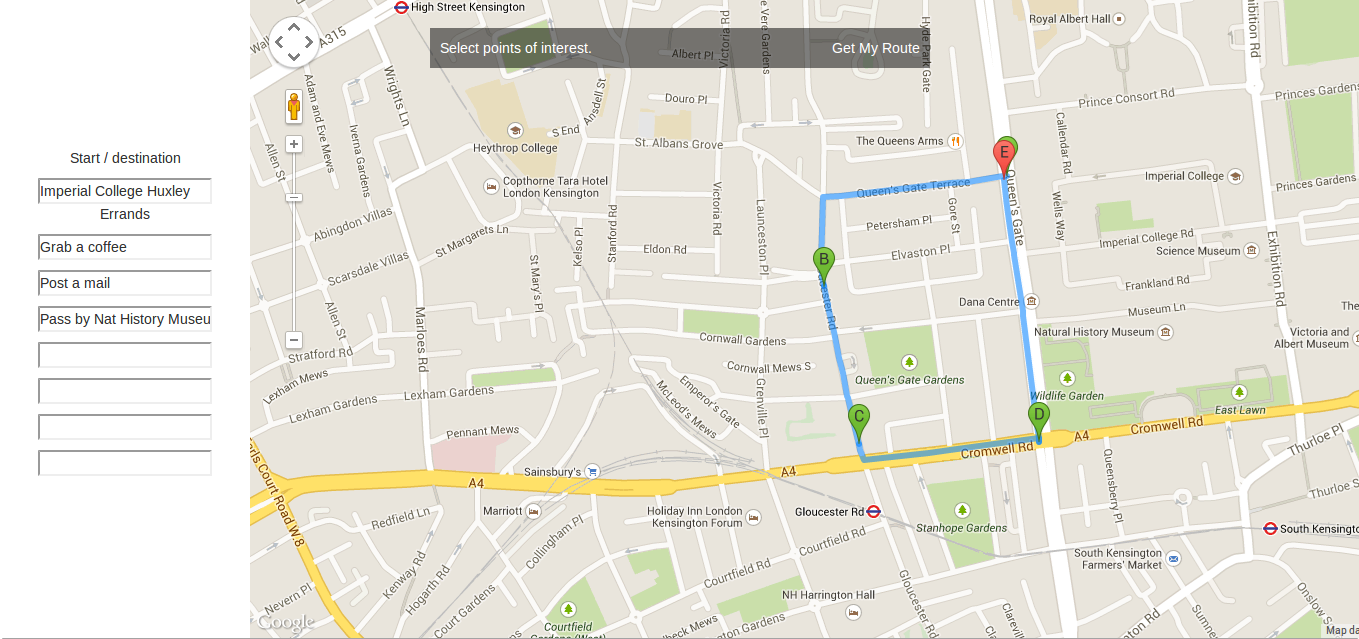
\includegraphics[scale=0.4]{hallway_q2.png}\\
Figure 2. UI the user will be presented with for this part of the test.
\end{center}

\newpage
\section*{Appendix B: Prototype}
\begin{center}
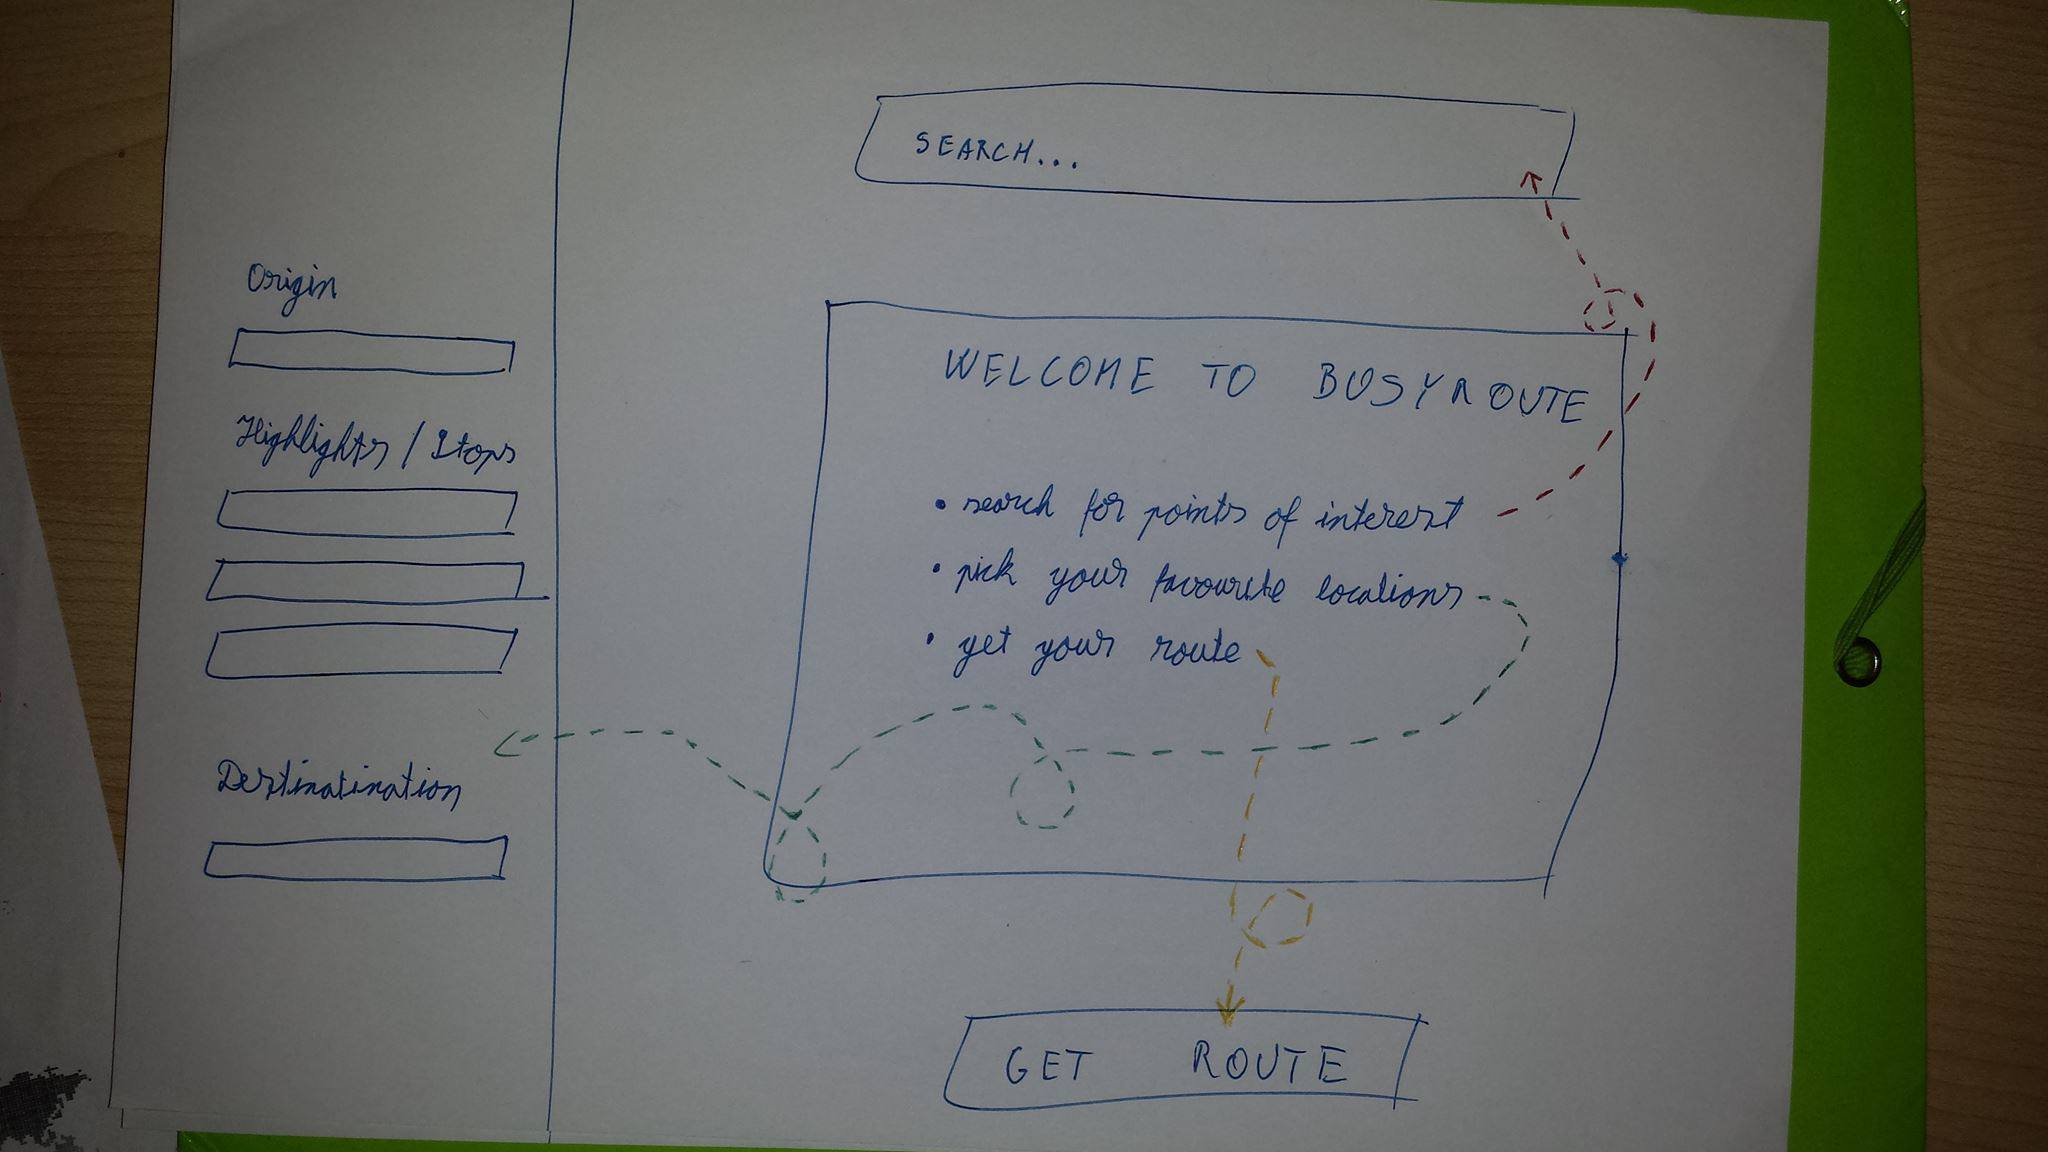
\includegraphics[scale=0.25]{proto_1.png}\\
Figure 3. Early paper prototype of the landing page.
\end{center}

\begin{center}
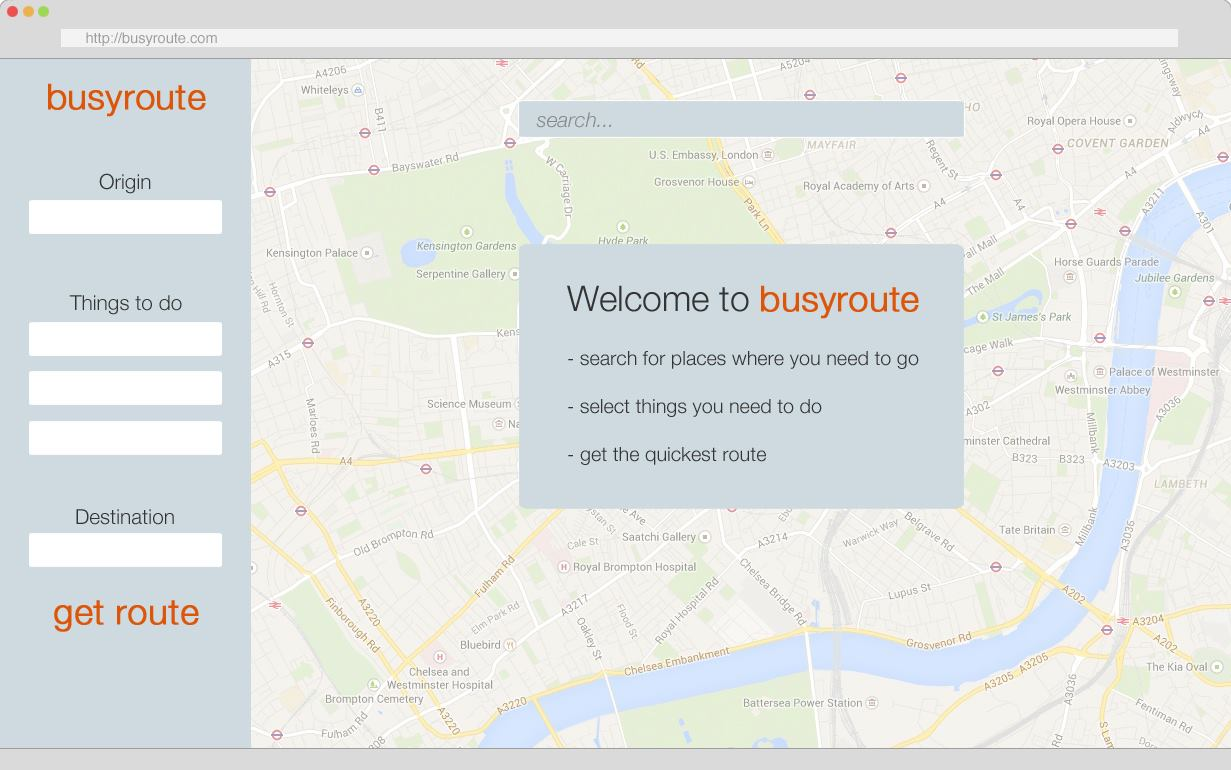
\includegraphics[scale=0.4]{proto_2.png}\\
Figure 4. Prototype of landing page.
\end{center}

\begin{center}
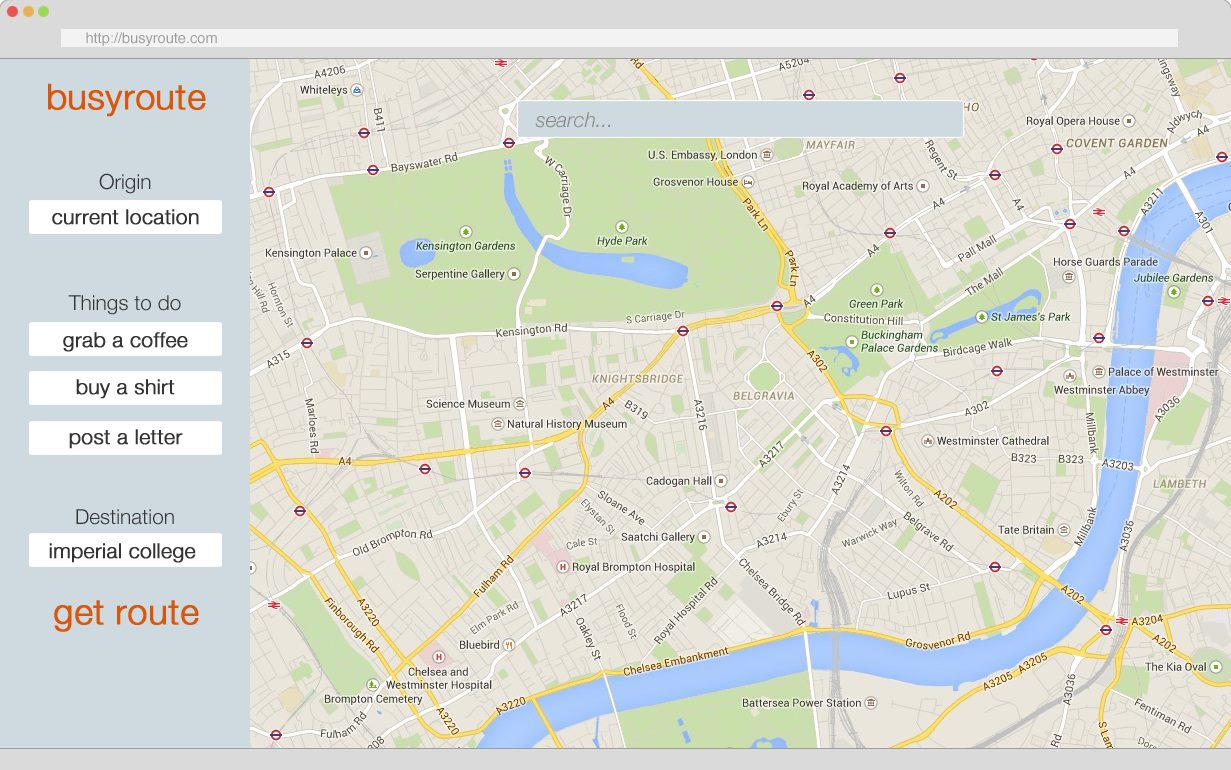
\includegraphics[scale=0.4]{proto_3.png}\\
Figure 5. Prototype of system whereby user enters his requirements.
\end{center}

\begin{center}
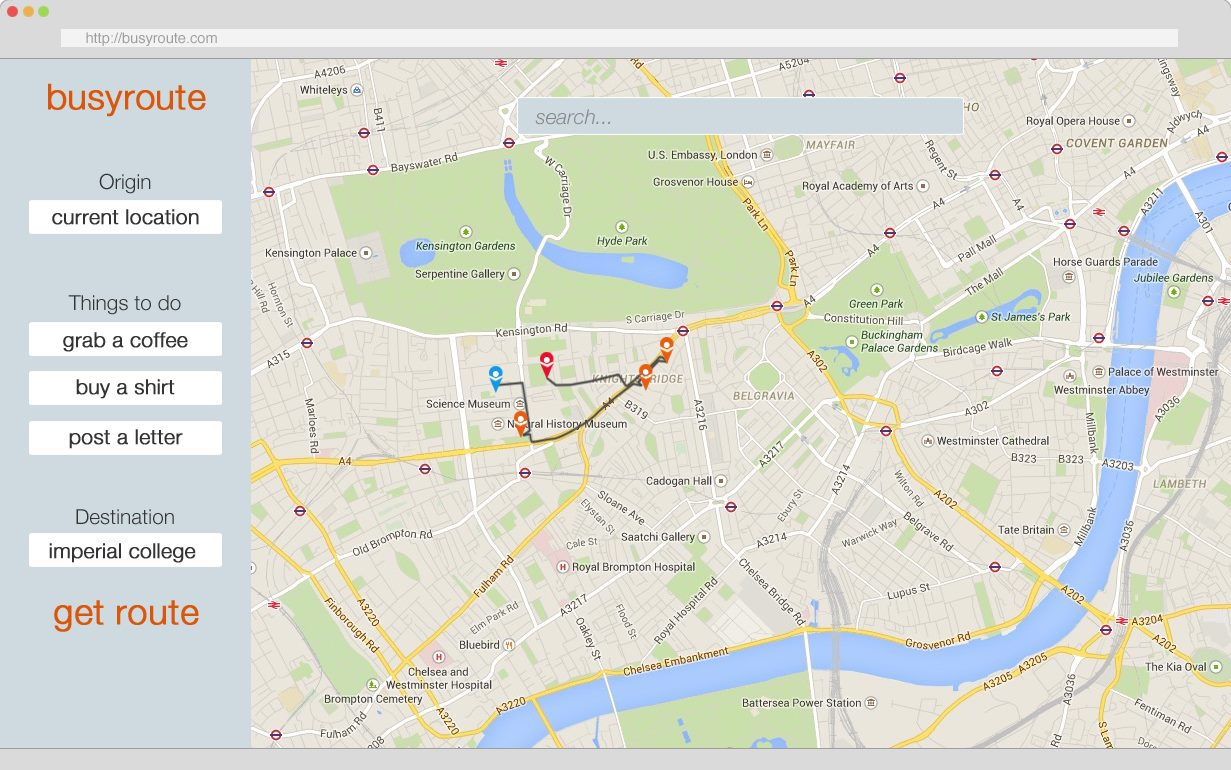
\includegraphics[scale=0.4]{proto_4.png}\\
Figure 6. Prototype of visualisation of the final route.
\end{center}

\newpage
\section*{Appendix C: Diagrams and Images}
\begin{center}
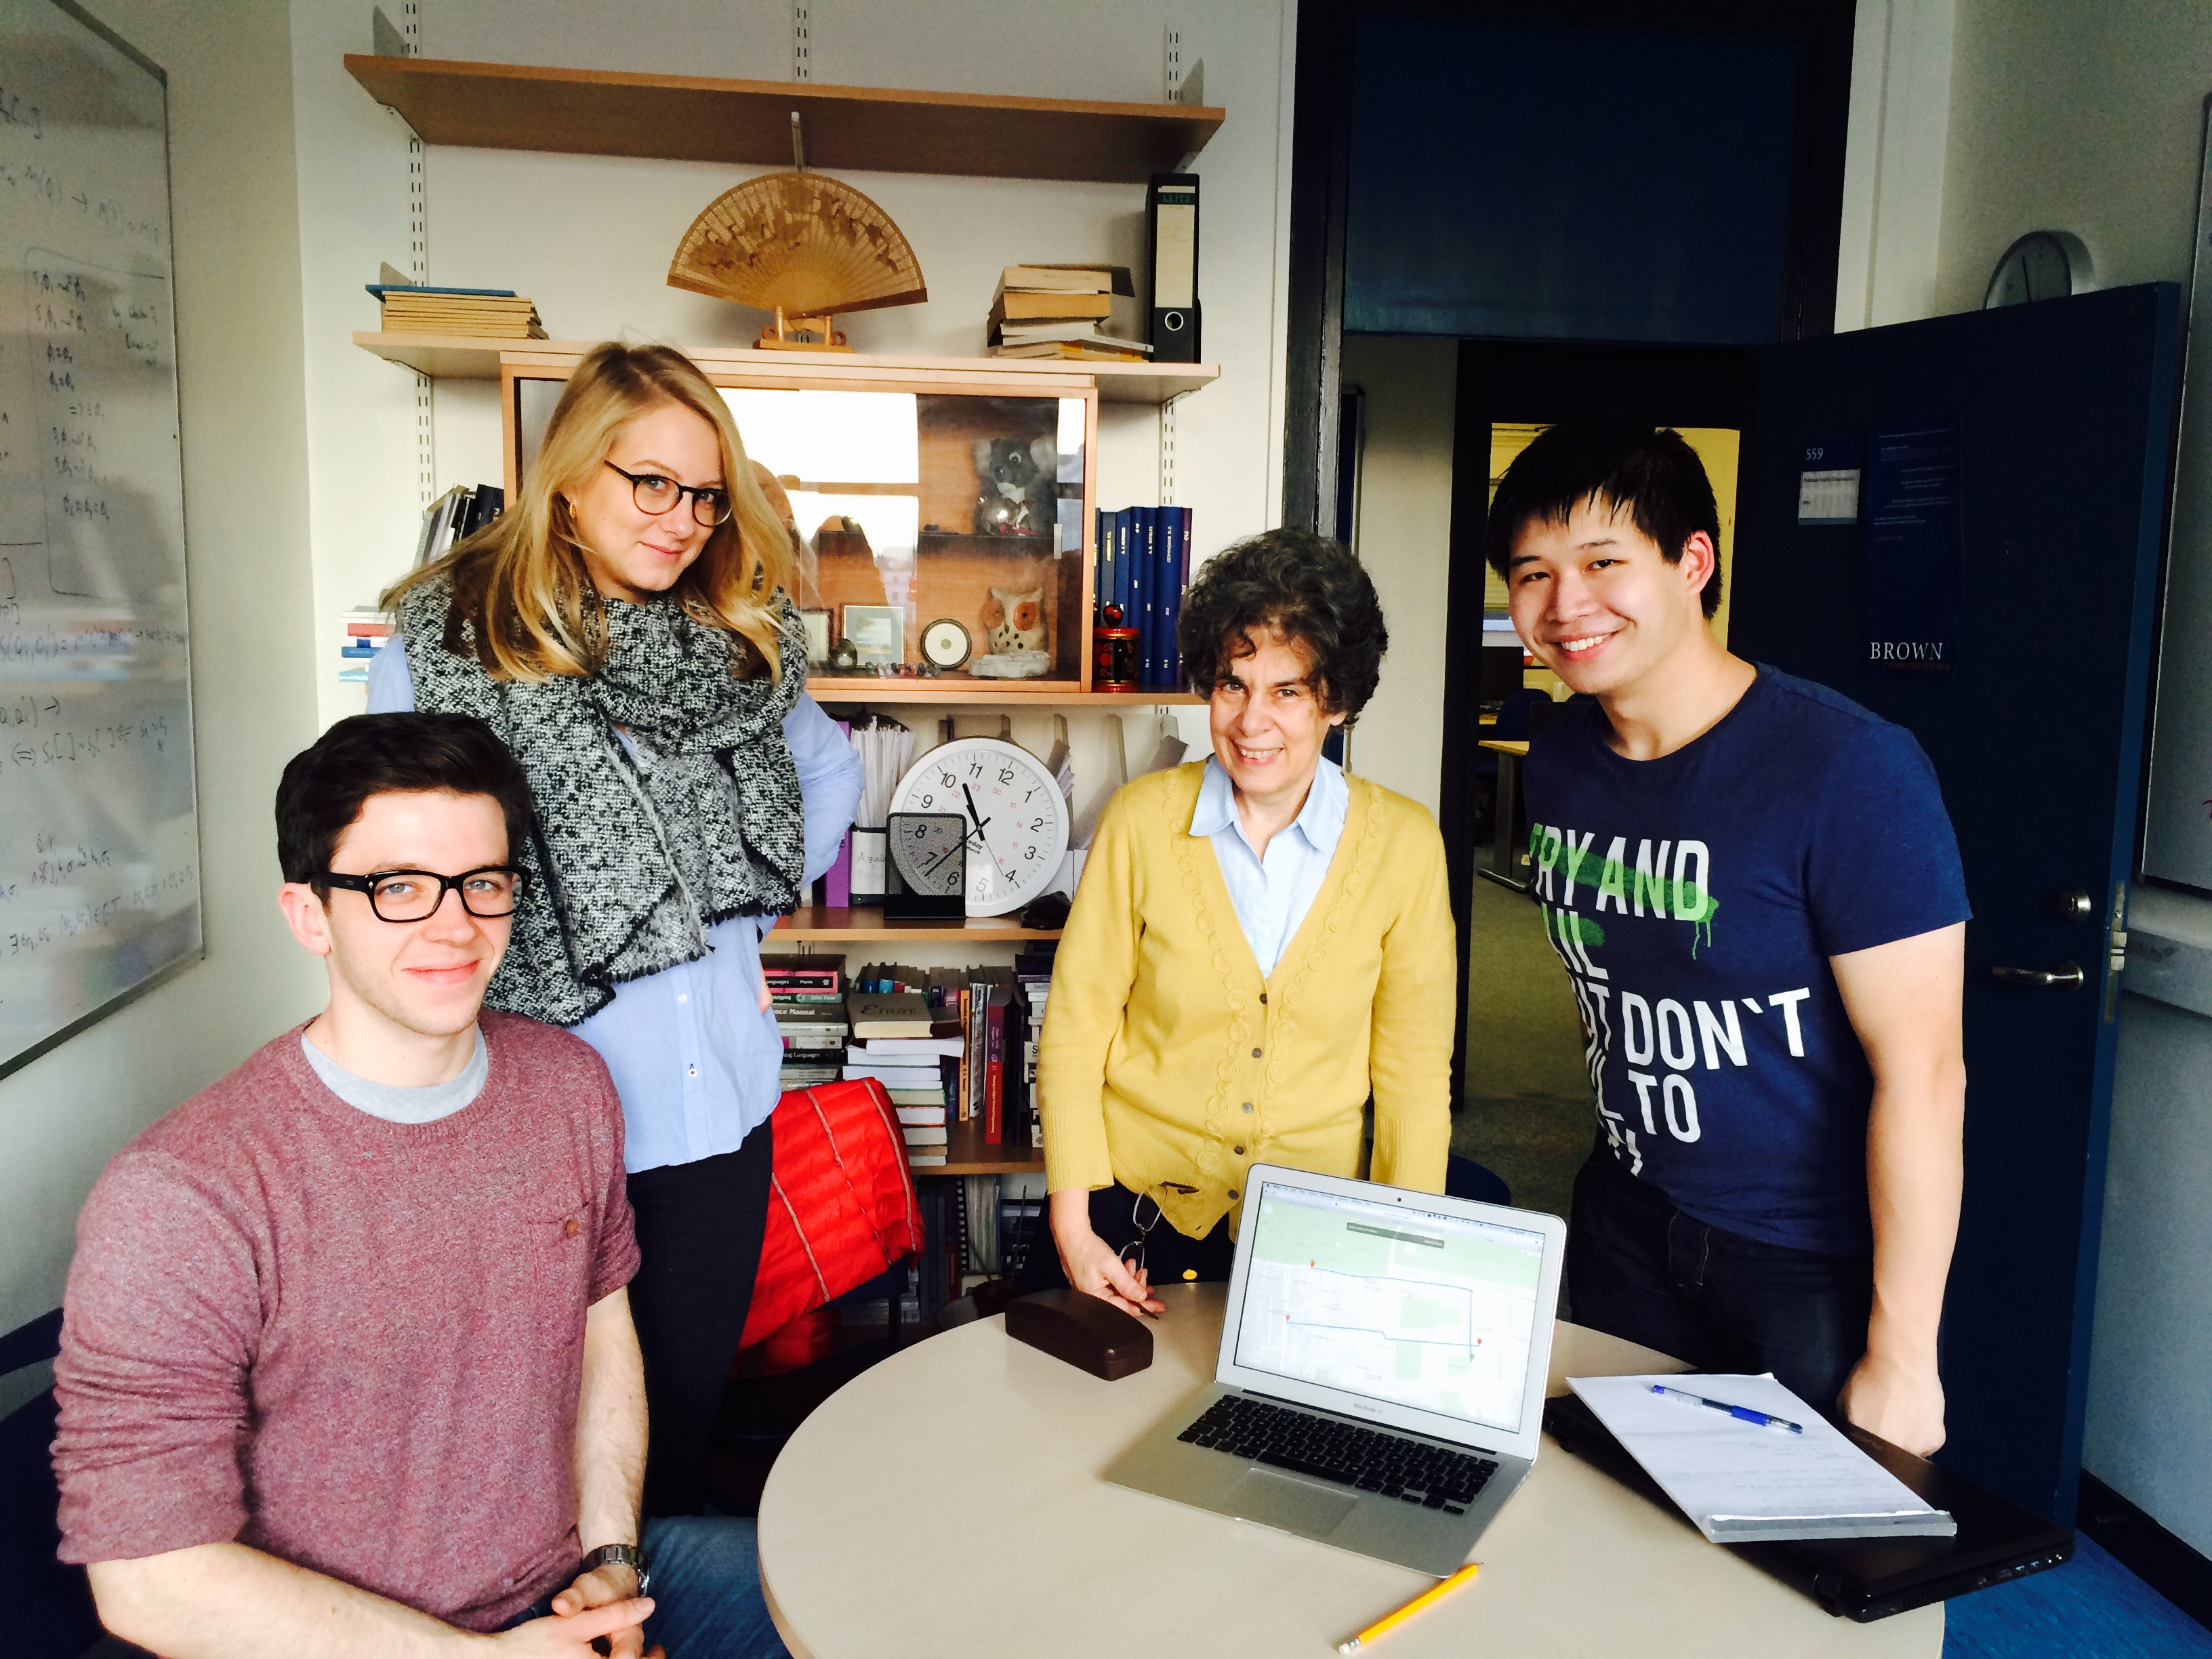
\includegraphics[scale=0.15]{sophia_x.jpg}\\
Figure 7. Sprint demo meeting with Project Supervisor (PS).
\end{center}

\end{document}